\subsection{Safety Assessment Process}
\label{subsec:process}

One of our goals is to transition the tools we have developed into use by the safety engineers who perform safety assessment on the avionics products. Therefore, we need to understand how the tools and the models will fit into the safety assessment and certification process.

ARP4754A, the Guidelines for Development of Civil Aircraft and Systems [ref. ARP4754A], has been recognized by the Federal Aviation Administration (FAA) as an "acceptable method for establishing a development assurance process" [ref. AC 20-174]. Figure~\ref{fig:plugin-arch}. from [ref. ARP4754A] demonstrates the ARP4754A process flow. The safety assessment process is a starting point of the integral processes, and is tightly coupled with the system development and verification processes. It is used to show compliance with certification requirements, and meeting a company's internal safety standards [ref. ARP4754A]. ARP4761, the Guidelines and Methods for Conducting Safety Assessment Process on Civil Airborne Systems and Equipment [ref. ARP4761], identifies a systematic means to show compliance. The guidelines presented in ARP4761 include industry accepted safety assessment processes (Functional Hazard Assessment (FHA), Preliminary System Safety Assessment (PSSA), and System Safety Assessment (SSA)), and safety analysis methods to conduct the safety assessment, such as Fault Tree Analysis (FTA), Failure Modes and Effect Analysis (FMEA), and Common Cause Analysis (CCA). 

\begin{figure}[h!]
	\vspace{-0.19in}
	\begin{center}
		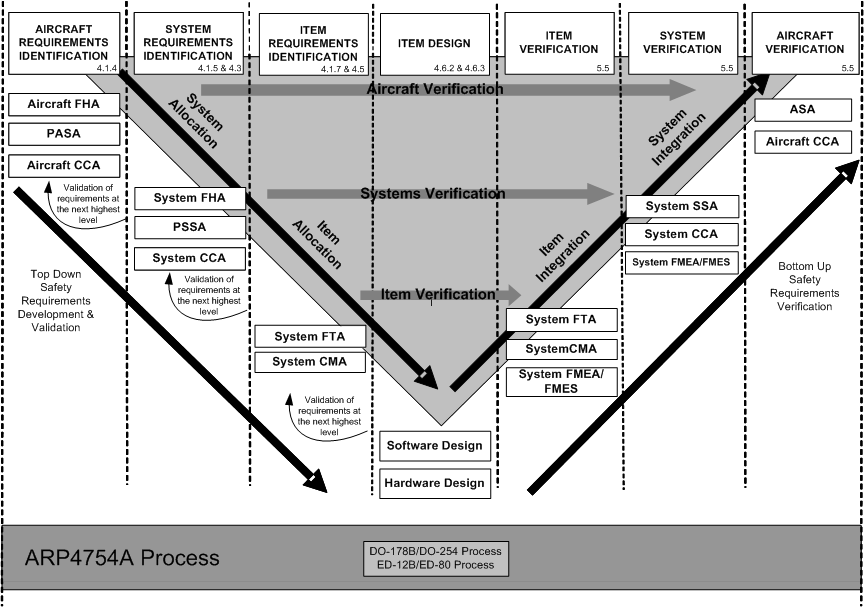
\includegraphics[trim=0 9 0 5,clip,width=1.0\textwidth]{images/ARP4754A_Process.png}
	\end{center}
	%\vspace{0.4in}
	\caption{ARP4754A Process(from ARP4754A ref)}
	\label{fig:arp4754a_process}
\end{figure}

A prerequisite of performing the safety assessment of a system design is to understand how the system works, primarily focusing on the integrity of the outputs and the availability of the product. The safety engineers then use the acquired understanding to construct the safety analysis artifacts, conduct safety analysis, and compare the analysis results with established safety objectives and safety related requirements. 

In practice, prior to performing the safety assessment of a system, the safety engineers are often equipped with fair amount of knowledge on how system works in general, but not necessarily with the specific system. Acquiring the knowledge on the content and behavior of a specific system has shown to be time consuming to get it right. For example, it took a safety engineer two solid days to understand how the software works in a Stall Warning System (a small system in comparison to a flight control computer). This is the same amount of time, if not more, as constructing the analysis artifacts and performing the analysis itself. In another example, coming up with the PSSA document for a horizontal stabilizer control system took a safety engineer more than a month to develop and multiple rounds of reviews involving system, software, and hardware engineers.

Using the same system design model to conduct both system design and safety analysis helps reduce the gap in comprehending the system behavior and transferring the knowledge between the design model to the safety analysis model. It maintains a living model that captures the latest state of the system design as the process flows per Figure~\ref{fig:plugin-arch}. It also allows all participants of the ARP4754A process to be able to communicate and review the system design using the "single source of truth". Industry practitioners have also realized the benefits and importance of using a system/safety model to generate the safety analysis artifacts, and a revision of the ARP4761 with model based safety analysis appendix is under way.

%Model Based Safety Analysis (MBSA) helps the above process by capturing the system architecture and functional behavior as well as failure mode and safety-relevant functional behavior in an augmented design model or separate safety model 

%ARP4761A MBSA Appendix draft, AIR6110, Rockwell white paper
%check Figure 7 of ARP-4754A for step by step process of the traditional approach


\begin{comment}
%Talks about the big picture, background, why we are doing this


\begin{itemize} 
\item Overview of the current/traditional safety assessment
Traditional process: V chart, starting from FHA to preliminary FTA to ...

\item Drawback/inefficiencies with the current safety assessment
The causal effect in the fault tree is manually come up by safety engineers after understanding the signal and function flow in the system/sw design documents for
the related functionality. 
The logical causal relationship is represented in a descriptive fault tree structure. 
It works well when the signals are processed in a sequential/linear fashion, but not when there are interactions/feedback loops that make the causal effect no longer linear?

\item Where our approach can help while other approaches cannot do as well
Out model uses the system architecture model 

\item How our approach can help: step by step process; inputs and outputs	

\end{itemize}


"working on safety analysis process. Strategy:
1. Check the example Mike Peterson did with stall warning
2. Come up with model in our end
3. See if we can catch anything missed by the fault tree, or help supply the fault tree analysis"
start process investigation by:
1. select the example from stall warning where mike has produced a fault tree from the document
2. independently model from the stall warning doc and try to:
get information from the fault tree that can build the structure of the fault tree
get information from the verification that can help trim/update the probability numbers of the fault tree
3. Compare the fault tree produced by Mike and the information supplied by our study, and see if we provide values to this study
Repeat this for an example fault tree from the white paper Mike sent

Process investigation
How should our model interact with the fault tree that Mike come up with? Any place we can work to create the tree for him? Or provide additional scenarios? Or validate the probabilities for his tree? Or SW/HW/Sys interactions that our approach captures that is hard to capture/verify using his approach?
How does the behavioral/interaction part of the document be modeled in the fault tree and in our model?
What findings from the safety process is driving the model/design updates, such as redundancy?
Would the AMASE modeling and analysis approach justify to make a conservative fault tree less conservative?
How the process steps are different from the process steps for ARP4761A MBSA?

With our process, do we have to use our tool/approach? Or other tools/approaches like xSAP could also work? What's the uniqueness of using our tool in this process? What's the benefit of this process in comparison to the current/traditional safety process?

"Documents to read:
- the white paper by Mike Peterson's group
- ARP4761A model based development supplement
- AIR 6110
- ARP4761
- ARP4754"
According to ARP4761A MBSA supplement draft, the MBSA model is called the Failure Propagation Model (FPM).
ARP4761A MBSA supplement identified some limitation of MBSA, including "it may be difficult to represent complicated Failed Conditions".
Check the simple example (Section 6) in ARP4761A MBSA

Answer from process point of view: why is our approach better than what's out there? What problem are we trying to solve?
Are we doing FPM (Failure Propagation Model) per ARP4761 MBSA?
MBSA section 6.2 shows a complex MBSA example

Give a detailed description of how fault tree is related to the AMASE nominal and faulty model, and the results from the AMASE verificaiton is relayed/fed bak to the fault tree

Check NFM reviewer comments
\end{comment}
